\documentclass[twoside,a4paper,11pt]{article}
\usepackage[a4paper,top=2.54cm,bottom=2.54
cm,left=3cm,right=3cm,marginparwidth=1.75cm ]{geometry}
\usepackage{graphicx}
\usepackage{multicol}
\usepackage{ragged2e}
\setlength{\columnsep}{1cm}
\usepackage[labelfont=bf]{caption}
\usepackage{fancyhdr}\fancyhf{}
\lhead{}
\rhead{\thepage}
\cfoot{}
\fancypagestyle{plain}{}
\usepackage[english]{babel}
\usepackage[utf8]{inputenc}
\usepackage{lipsum}
\usepackage[
backend=biber, style=numeric, sorting=none
]{biblatex}
\addbibresource{./refs.bib}
\usepackage{lmodern}

\usepackage{hyperref} 

\title{Gamification of Electric
 Circuits Education}
\author{Nour Gaser , Hazem Gamal , Rokaia Medhat, Mohammed Hussein  }

\date{December 2022}

\begin{document}
\begin{center}
\LARGE
\textbf{Gamification of Electric Circuits Education}
\newline
\hfill \break
\large
Nour Gaser, Rokaia Medhat, Mohamed Hussein \& Hazem Gamal
 \newline
\hfill \break
\normalsize
Misr University for Science and Technology -\textit{ MUST}, College of Computers and Artificial Intelligence Technology - \textit{CAIT}, Department of Computer Science - \textit{CS}

\hfill \break
\normalsize
\large 2022-2023   
\end{center}
\pagestyle{fancy}
\setlength{\headheight}{1.5cm}.

\centering
\hrule
\subsection*{Abstract} 
\footnotesize
\centering
In the current academic and research scene, the topics of embedded systems and robotics are of high interest and need, though learners often find that they lack the needed fundamentals in electronics to conduct their projects and research. This project proposes a visual education solution for fundamental electronics and electric circuit simulation, by harvesting the concepts and technologies of gamification, game design, and puzzle design. 

\hfill \break
\hrule

\begin{multicols}{2}
\footnotesize
\justifying
\section{Introduction}

Most students regardless of their scientific level often find the idea of learning about circuits a very intimidating one, it is a topic often associated with the idea of being difficult. And that applies to both the theoretical side and the practical side of the learning process, it is a demanding topic that requires the student to have an understanding in multiple fields such as mathematics and physics. 

Students from all levels may find difficulties in understanding topics such as voltage, current, and how these properties are affected by different components in a circuit. This can be seen for example in the research administered by Carol Bowman and Gordon J. Aubrecht, II \cite{1}, they found that students find the concept of voltage very confusing, and that is due to the fact that students first start by learning about current, then when they start learning about voltage they apply the idea of flow which applies to current, as a result students start confusing the two concepts together, and that it is despite careful texts which attempt to clarify the difference among the two.

Another challenge that students face nowadays is their very short attention spans. Students need something engaging and entertaining to keep them interested, traditional methods such as long lectures, and large textbooks, while informative, but they lack the attention grabbing element, students get bored and lose interest. According to Neil A. Bradbury \cite{17} several institutions have brought down the length of lectures to only 15 minutes. This is based on the belief that a lecture any longer than 15 minutes is not going to be effective for students.
\vfill
\section{Gamification as an approach}
There have been a lot of different definitions for gamification with different perspectives from different authors. Dixon, Khaled, and Nacke suggested defining “gamification” as “the use of game design elements in non-game contexts”. van Grove(2011) \cite{2} ”Gamification is to change something that is not a game through a game or its elements.”. MacMillan (2011) \cite{3} ” Gamification, defined as the use of game mechanics, dynamics, and frameworks to promote desired behaviors”. So we could simply say that gamification is the systematic process of applying game mechanics to non-game contexts to make difficult tasks more enjoyable. 

Gamification aims to make an otherwise dull experience tolerable, if not desirable. Good game design must be practiced, otherwise either the essence of the topic will be lost (preserve the essence of the topic), or the experience will just be dull, or even leaving a negative impression on the topic.

\section{Our proposed solution}

Our proposed solution is to develop an educational puzzle game, whose player can both enjoy an entertaining experience regardless of their scientific interest level, all the while implicitly gaining valuable experience and knowledge in electric circuits design, where they can opt in for a more academic learning experience through references to external materials, data-sheets, and circuit schematics designed to encourage real-life experimentation, and allow for academic instructors and supervisors to supplement their coursework and practical assignments with select (or all) sections of the game.
\section{Preliminary study}
\subsection{Literature review}
In order to determine whether our solution would be useful or not, as well as how to approach it, we need to review previous attempts at gamifying the educational experience. Therefore, we conducted a literature review of most of the current relevant works. The summary of that is as follows: \\
\begin{itemize}
    \item an experiment done on a sample of 294 students registered in the first year and first semester in an electromechanical engineering course shows that traditionally, in math classes, the attendance
    is low specially in first year but in the classes where gamification was used, attendance saw a considerable increase in both theoretical and practical classes and the rate of students who dropped out was lower than
    the previous years. \cite{26}
    \item According to statistics represented by Educational Evaluation National Institution (EENI), 22.8\% of the students form the Andean region and 18.3\% from the coast have insufficient grades in areas that include the study of science (Physics, Chemistry and Biology). From this point
    this study proposes a solution by developing a physical mobile application that implements the methodologies of gamification and increased reality with the intention of improving creativity and
    academic performance of the students. \cite{27}
    \item a study was conducted on 43 students in secondary vocational engineering. There were two conditions, the traditional
    learning condition, and a virtual lab one. The post-test results show that the virtual-lab condition students obtained significantly higher overall
    scores, than the participants in the traditional condition. Virtual-lab students also scored higher on the conceptual items. \cite{25}
    \item A study for comparing the effectiveness of a computer simulation
    and a hands-on activity on learning electric circuits shows that incorporating any form of interactive learning can be beneficial
    and will increase the quality of the students’ learning experience, regardless of whether it is a hands-on experience or a computer simulated one. \cite{24}
\end{itemize}
\textbf{For the full literature review see \cite{29} section 2.1.}
\subsection{Survey}
We also conducted a survey in order to see whether our solution would be helpful to students, as well as to exactly determine the challenges that they face during their studies. The next few figures show the students' responses to the following questions:
\begin{itemize}
    \item How would you rate the difficulty of your electric circuit-related courses?
    \item Please describe any challenges that faced you while circuit simulation software.
    \item Would you be interested if there was a puzzle video game that attempts to simplify electric circuit education (including simulation) and make it entertaining? 
\end{itemize} 
\begin{center}
    \includegraphics[width=0.5\textwidth]{Screenshot from 2022-12-17 10-10-45.png}
    \captionof{figure}{ Rating the difficulty of electric circuits related sources through academic programs} 
\end{center}

\begin{center}
    \includegraphics[width=0.5\textwidth]{Screenshot from 2022-12-17 10-11-29.png}
    \captionof{figure}{The students interest in applying a gamification solution } 
\end{center}

\raggedright\textbf{Challenges that faced the students when using circuit simulation software}
\begin{itemize}
    \item The user interfaces are hard to deal with.
    \item Sometimes there are too many options and the students don't know exactly which type of component is the one they are looking for.
    \item Configuring and running simulations.
    \item "The guidelines of using the app wasn't specific and in some applications such as Proteus the usage of the application wasn't logical for me". 
    \item "They werent very realistic, I had challenges while using them they weren't that simple to use, or even to get it, the accuracy wasn't high, it lagging some time, and performance was too low."
\end{itemize}

\textbf{For the full survey see \cite{28}.}

\section{Methodology}

The game will run on the unity game engine utilizing a lot of its features. As for the simulation of the circuits we will use the C\# library SpiceSharp. SpiceSharp is a circuits simulation library that is compatible with the Berkeley Spice simulator. The player will interact with the game through its user interface, those interactions could be navigational interactions to transition from one menu or scene to another, or they could be gameplay interactions when playing a level. Then in order to complete a level the player needs to achieve some goals that are introduced at the beginning of the level. The circuits submitted by the player is then simulated using SpiceSharp and the results are sent back to the game, the game then decides whether the goals were achieved or not.

\begin{center}
    \includegraphics[width=0.5\textwidth]{System Design & Architecture.png}
    \captionof{figure}{System Architecture} 
\end{center}
    
\section{Results} 
\subsection{The game}
A 2D puzzle game consisting of the following elements, with each element's traditional education rough/most similar counterpart:
\begin{itemize}
    \item \textbf{Backstory}: set in a fictional world which grabs the attention of the player and incentivizes them to continue playing the game to learn more about the story. \textit{No counterpart in traditional education.}
    \item \textbf{Main character}: guides the player through the game, giving them hints, and interacting with them, creating an emotional attachment. \textit{Counterpart in traditional education: tutors}. 
    \item \textbf{Puzzle tree}: contains a tree of available puzzles in a hierarchical tree-structure, which each node representing playable puzzle. \textit{Counterpart in traditional education: curriculums}.
    \item \textbf{Mini-games}: offer a repetitive challenge where the player can "farm" rewards, implicitly teaching the player real life electronics skills which would only be gained through repetition. For example: reading resistor color-code bands quickly. \textit{Counterpart in traditional education: practical repetitive-practice}.
    \item \textbf{Collection}: a collection of everything the player has won (learned) so far in the game, presented as an in-game book (encyclopedia) containing references to real learning materials, theoretical explanations, as well as data sheets, schematics, and a database of components, which the player unlocks gradually as they progress through the puzzle tree. \textit{Counterpart in traditional education: textbooks \& manufacturer data sheets}.
    \item \textbf{Progression and rewards}: by combining the player's progress on the puzzle tree, their collection, and farmed rewards from the mini-games, the player can "upgrade" the main character, helping them along, and unlocking new chapters of the story. \textit{No counterpart in traditional education.}
    \item \textbf{Sandbox mode}: a free-form "lab" scene where the player has access to an unlimited number of the components which they've unlocked so far to experiment with as they please. \textit{Counterpart in traditional education: simulation software}.
\end{itemize}
\begin{center}
    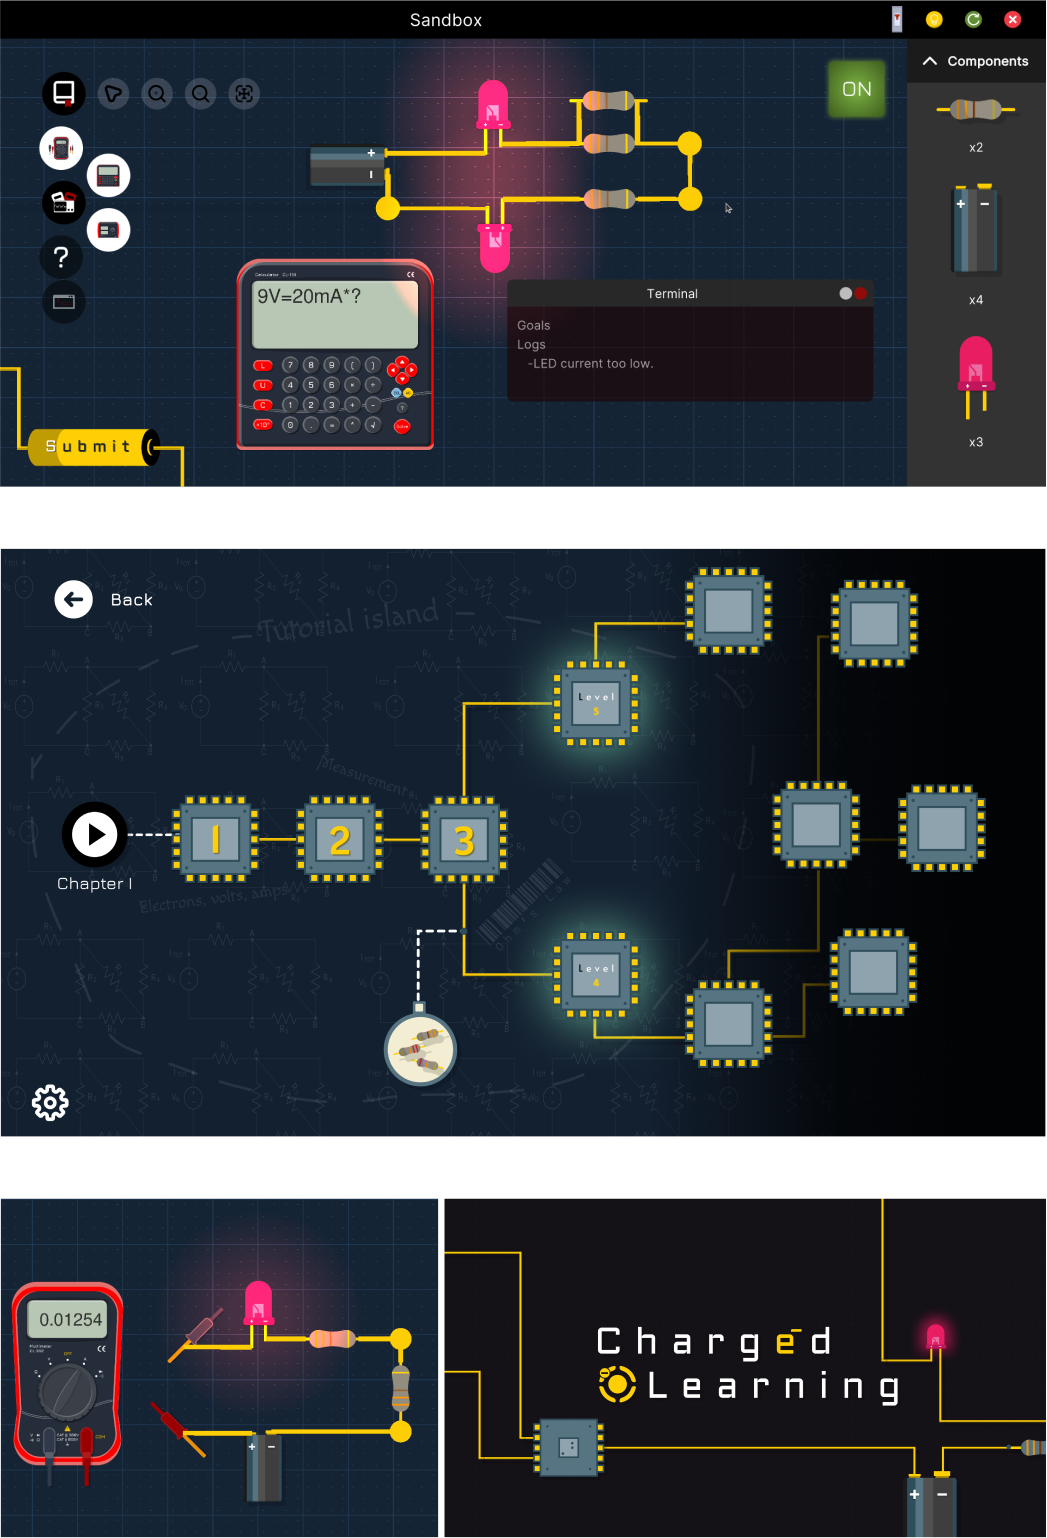
\includegraphics[width=0.5\textwidth]{images/game_screenshots.png}
    \captionof{figure}{screenshots from the game} 
\end{center}


\subsection{Follow up with survey-takers who agreed to test the game (closed-testing and public testing)}
 \textbf{Closed-testing currently ongoing, with public-testing planned soon}. We have been following up with the survey-takers who agreed to test the game. We have conducted closed testing with a small group of students and have received positive feedback. The students have found the game to be engaging and challenging, and they have learned a lot about electric circuits.

 We are currently working on completing the game and will be conducting public testing in the near future. We will then publish a separate paper with the results of the public testing, including the game's impact on students' grades and understanding.
 
 Due to unplanned budget issues and running overtime for the project's due date, we will not be able to conduct public testing as soon as we had hoped. However, we are committed to completing the game and conducting public testing as soon as possible.
 
 We appreciate the patience and understanding of the survey-takers who agreed to test the game. We are excited to share the game with students in the near future.
 
  

 \section{Conclusion}
 In conclusion, we developed a puzzle video game to teach students about electric circuits. The game was designed to be engaging and challenging, and it incorporated a variety of gamification elements. Due to limited budget and time, only 75\% of the originally planned features were implemented. However, we are still working on adding the rest of the features. We will also be conducting testing to ensure that the game is both educational and fun.
 
 We believe that this game has the potential to be a valuable tool for teaching students about electric circuits. We are excited to continue working on the game and to share it with students in the future.
 
 Here are the challenges that we faced, the lessons that we learned, and our plans for the future:
 
 \subsection*{Challenges}
 \begin{itemize}
    \item Learning about electric circuits in order to make sure that our simulation was accurate.
    \item Designing and implementing the system in C\# using various design patterns.
\end{itemize}
\subsection*{Lessons Learned}
\begin{itemize}
     \item Clean coding principles
     \item Agile (Scrum) project management
     \item Teamwork between engineers, programmers, artists, and game designers
     \item Various algorithms like linear interpolation for animation, and graphs for electric circuits connections.
\end{itemize}
\subsection*{Plans for the Future}
\begin{itemize}
     \item Add more components to the game, such as capacitors, inductors, transistors, and various ICs.
     \item Add minigames to aid certain skills, such as reading resistor values and datasheets.
     \item Add a textbook in the game (in-game encyclopedia).
     \item Public testing
     \item Polish, marketing, and publishing on Steam
 \end{itemize}
 
 We are excited to continue working on this project and to share it with students in the future. We believe that this game has the potential to be a valuable tool for teaching students about electric circuits.
 
\printbibliography
\end{multicols}
\end{document}
